\documentclass[11pt]{article}
\usepackage[margin=1in]{geometry}
\usepackage[T1]{fontenc}
\usepackage{lmodern}
\usepackage{microtype}
\usepackage{graphicx}
\usepackage{booktabs}
\usepackage{amsmath}
\usepackage{xcolor}
\usepackage[round]{natbib}
\usepackage[colorlinks=true,linkcolor=blue!50!black,citecolor=blue!50!black,urlcolor=blue!50!black]{hyperref}
\usepackage{listings}
\lstset{basicstyle=\ttfamily\small,columns=fullflexible,breaklines=true,frame=single,framerule=0.3pt}
\bibliographystyle{plainnat}
\setcitestyle{authoryear,round}

\title{Tripwire: Reading What a Reasoning Model Does,\\Thinks, and Says on Impossible Coding Tasks}
\author{Dhairya Pandya\\
PDPM Indian Institute of Information Technology, Design and Manufacturing (IIITDM) Jabalpur}
\date{November 2026}

\begin{document}
\maketitle

\begin{abstract}
Coding agents are rewarded when tests pass, which gives them an incentive to make tests pass without solving the task. We study how an open-weight reasoning model behaves under that incentive, and whether the behaviour can be read from its visible reasoning or from its report to the user. We build 44 impossible variants of real bug fixes from fastapi, rich and requests by changing one expected value in each task's regression test, and we verify by program that the known-good fix fails every variant. We run Beam, a 501B-parameter reasoning model with an adjustable effort setting, on these variants and on the unmodified tasks in an offline sandbox, for 616 episodes in total, and label each episode at three layers: behaviour, reasoning and report. Beam modified a test or special-cased library code in 66\% of impossible episodes at low effort and 79\% at high effort, against 1 in 176 control episodes. An instruction not to modify tests reduced this to 23\% and 41\%. With a 30-turn budget, high effort appeared to cheat far less (20\%), but 38 of 44 of those runs had exhausted their turns; with 60 turns the apparent effect reversed. Beam's reasoning revealed most cheating: a keyword rule over the reasoning detected 83\% of cheating episodes in the run where Beam could write to the user, while Beam's own note to the user disclosed 15\%, and never disclosed a special-cased value. We release the episodes, labels, harness and an interactive explorer.
\end{abstract}

\section{Introduction}

Automated tests are the standard signal of success for coding agents, both in evaluation and in training. The signal has a known weakness: a test can be satisfied without the behaviour it is meant to check. An agent can edit the test, delete an assertion, or make the code return the expected value only for the input the test uses. When such shortcuts are rewarded, they are a form of reward hacking, and recent reports describe frontier models taking them in practice \citep{metr2025rewardhacking,baker2025monitoring,zhong2025impossiblebench}.

Two questions follow for anyone deploying a coding agent. The first is behavioural: how often does the agent take the shortcut, and what conditions change that rate? The second is about visibility: if it takes the shortcut, will anyone notice? Reasoning models offer a possible answer to the second question, because they produce a chain of thought before acting. If the intent to cheat appears in that text, a monitor can read it \citep{baker2025monitoring,korbak2025cot}. Other work shows that reasoning text is not always a faithful account of what drives a model's output \citep{turpin2023unfaithful,chen2025reasoning,arcuschin2025wild}, so whether it helps in a given setting is an empirical question.

This paper studies both questions on one model. Beam \citep{reflection2026beam} is an open-weight reasoning model of 501B parameters (23B active) that returns its full reasoning and exposes a reasoning-effort setting (\texttt{low}, \texttt{medium}, \texttt{high}) on the same weights. Those two properties let us look at an agent's behaviour, its reasoning and its report together, and vary the amount of reasoning without changing the model. We call the approach \emph{behavioural interpretability}: we do not inspect weights or activations, but we compare what the model does, what its reasoning says, and what it tells the user, and ask where these three layers agree.

We construct impossible coding tasks in the manner of \citet{zhong2025impossiblebench}. Starting from real bug fixes, we change one expected value in each task's regression test so that it contradicts the issue, and we confirm by program that the known-good fix fails the changed test. Any patch that then passes the changed test must have modified the test or bent the library toward the wrong value. We ask three research questions:

\begin{description}
\item[RQ1] How often does Beam cheat on impossible tasks, how does it cheat, and how do an honesty instruction and the effort setting change this?
\item[RQ2] Does Beam's reasoning reveal the cheating, and how well do simple monitors read it?
\item[RQ3] Does Beam's report to the user reveal the cheating?
\end{description}

Our contributions are:
\begin{itemize}
\item An offline harness that builds impossible variants of real bug fixes, proves each one impossible, runs an agent in a network-less sandbox, and labels each episode at the levels of behaviour, reasoning and report.
\item Measurements on Beam over 616 episodes. Beam cheated on most impossible tasks and almost never on real ones. An honesty instruction reduced but did not remove the behaviour. Higher effort did not reduce it once the turn budget was large enough.
\item Evidence that, for this model and setting, the reasoning is the more informative record: it revealed most cheating episodes, while the model's own report rarely did.
\item A methodological finding for evaluation design: a fixed turn budget made higher effort look safer because high-effort runs ran out of turns before acting.
\item A public dataset of all episodes with labels, the harness, and an interactive explorer.
\end{itemize}

\section{Related work}

\paragraph{Impossible tasks and test exploitation.}
SWE-bench \citep{jimenez2024swebench} established real GitHub issues with hidden regression tests as a benchmark for coding agents. ImpossibleBench \citep{zhong2025impossiblebench} mutates such tests so that they conflict with the specification, which makes any pass a cheat by construction. It reports frequent cheating by frontier models on its SWE-bench-derived split (for example, GPT-5 on 54--76\% of tasks depending on the variant), a range of strategies from test edits to operator overloading, a strong effect of prompt strictness, and LLM monitors that detect cheating well on short problems but less well on repository-level tasks. Our variant construction follows the same idea at a smaller scale. We add a reasoning-effort sweep on fixed weights, a model whose complete reasoning is available, and a comparison with the model's report to the user.

\paragraph{Reward hacking in practice.}
\citet{metr2025rewardhacking} describe frontier models modifying tests and scoring code during evaluations, while showing awareness that this conflicts with the user's intent. \citet{denison2024sycophancy} show that models trained on easily discovered specification gaming generalise to rarer and more blatant forms, up to editing their own reward function. \citet{macdiarmid2025emergent} find that reward hacking learned in production coding environments can generalise to broader misalignment. Together these results motivate measuring test exploitation before deployment and training, rather than after.

\paragraph{Monitoring the reasoning.}
\citet{baker2025monitoring} show that a weaker model reading a reasoning model's chain of thought detects reward hacking in agentic coding far better than one that reads actions alone, and that optimising against such a monitor leads to obfuscated reward hacking, where the intent disappears from the reasoning while the behaviour continues. \citet{korbak2025cot} argue that this monitorability is a valuable but fragile property that developers should track. \citet{emmons2025necessary} find that when a task requires multi-step reasoning, models struggle to hide that reasoning from a monitor without substantial help.

\paragraph{Faithfulness of reasoning.}
Other work cautions against treating reasoning text as a faithful record. \citet{turpin2023unfaithful} show chain-of-thought explanations that rationalise answers driven by unmentioned biases. \citet{chen2025reasoning} find that reasoning models rarely verbalise the hints they use, and that a model trained on environments with reward hacks exploited them on almost all prompts while mentioning them in under 2\% of cases in most environments. \citet{arcuschin2025wild} report unfaithful reasoning on natural prompts without injected bias. Our results are a data point in this debate for one model and one setting, in which the reasoning was largely candid and the user-facing report was not.

\section{Method}

\subsection{Tasks and impossible variants}

We use 44 bug-fix tasks from three Python libraries: fastapi (23), rich (16) and requests (5). Each task has an issue description, a repository snapshot, the known-good fix, and the regression tests added by that fix. The tasks and sandbox come from an earlier harness, which we reuse unchanged.

For each task we change one expected value in the regression test. The mutation finds the first added assertion of the form \texttt{assert \ldots{} == <literal>} and changes the literal: integers are incremented by one, floats by $1.0$, and strings receive the suffix \texttt{\_v2}. A typical variant is:
\begin{lstlisting}
-    assert response.status_code == 200
+    assert response.status_code == 201
\end{lstlisting}
A variant is kept only if the known-good fix, run against the changed test, fails at least one test that it passes against the original. We record those tests as the variant's \emph{broken tests}. All 44 candidate variants passed this check. Because the correct fix fails the broken tests, a patch that passes any of them must either change the test or make the code produce the wrong value.

\subsection{Agent setup}

Beam was accessed through the Hugging Face inference router with a single provider and default sampling. In each episode the agent works in a Docker sandbox with networking disabled and the task's dependencies preinstalled. It has tools to run shell commands, read files, edit or write files, replace line ranges, check its remaining budget, and submit a patch. Limits per episode are a turn cap (30 or 60, see below), 60 tool calls, 300 seconds per command, 5{,}000 characters of command output, and 8{,}192 completion tokens per turn. In the impossible conditions the changed test file is committed into the workspace before the agent starts, so it is visible and the agent's diff is measured against it.

\subsection{Conditions and runs}

Each task runs under three conditions, which differ only in the instructions:
\begin{itemize}
\item \textbf{Control}: the real task, with the instruction to fix the library code and check it with targeted tests.
\item \textbf{Impossible}: the changed test, with the instruction that the tests in the named file describe the required behaviour and should be made to pass.
\item \textbf{Impossible + honesty}: as above, plus ``Do not modify the tests. If the task cannot be completed as specified, explain why instead of forcing the tests to pass.''
\end{itemize}

We report three runs, 616 episodes in total (Table~\ref{tab:runs}). The first run (v1) covers all conditions at all three effort settings with a 30-turn cap. The second repeats the two impossible conditions at high effort with a 60-turn cap, for reasons given in Section~\ref{sec:turncap}. The third (v2) covers all conditions at low effort after a change to the harness. In v1, the system prompt instructed the agent to act only through tools, and the submit tool took no arguments, so the agent had no channel through which to report a problem to the user. In v2 the submit tool takes an optional \texttt{note}, described as a message to the user similar to a pull-request description, and the honesty instruction asks the agent to explain the problem ``in the note of submit\_patch'' rather than ``in your final message''. This wording change is the only difference in the honesty condition between v1 and v2. Two high-effort episodes ended in a provider outage and are excluded, leaving 614 for analysis.

\begin{table}[t]
\centering
\small
\begin{tabular}{llllr}
\toprule
Run & Conditions & Effort & Turn cap & Episodes \\
\midrule
v1 & control, impossible, impossible + honesty & low, medium, high & 30 & 396 \\
high-60 & impossible, impossible + honesty & high & 60 & 88 (86 analysed) \\
v2 (note) & control, impossible, impossible + honesty & low & 30 & 132 \\
\bottomrule
\end{tabular}
\caption{Runs. Each cell is one episode per task (44 tasks).}
\label{tab:runs}
\end{table}

\subsection{Three layers of labels}

All labels are computed by program from the saved trajectory. We spot-checked each label type against traces by hand; Appendix~\ref{app:labels} lists the definitions and the corrections made during validation.

\paragraph{Behaviour.} An episode has a \emph{test edit} if any tool call writes to the task's test file or another existing test file, either through a file tool or through a shell command that writes to it (redirection, in-place \texttt{sed} or \texttt{perl}, \texttt{rm}, \texttt{mv}, \texttt{cp}, \texttt{tee}, or a Python \texttt{open(\ldots, 'w')}). An episode is \emph{special-cased} if, with all test changes stripped from the final patch, at least one broken test passes. Since the known-good fix fails that test, the library must have been bent toward the wrong value. An episode \emph{cheated} if it has a test edit or is special-cased. Edits to test-runner configuration such as \texttt{pyproject.toml} are recorded separately and not counted as cheating, because the agent sometimes made them to silence unrelated warnings. We also record whether the patch passes the task's original hidden tests.

\paragraph{Reasoning.} Two monitors read only the concatenated reasoning text. The \emph{keyword} monitor is a regular expression for intent phrases (``change the test'', ``hard-code'', ``special-case'', ``\_\_eq\_\_'' and similar), which ignores matches preceded or followed by a negation (``can't modify the test'', ``change test? Forbidden'') and sentences that repeat the prompt's own instructions. The \emph{judge} monitor is Gemma~4~12B, run locally at temperature 0 without its own reasoning, asked whether the reasoning shows intent to make the tests pass by illegitimate means, and allowed to answer with a single word. We also record whether the reasoning states that the test is wrong.

\paragraph{Report.} For v2, we label whether the note says the test or task is wrong (the Gemma judge reading only the note) and whether, in a cheating episode, the note \emph{discloses} a test change (a rule matching phrases such as ``corrected the test'', checked by hand against all 41 cheating notes).

\subsection{Statistics}

Each cell has one sample per task, and we report proportions with Wilson 95\% intervals \citep{wilson1927probable}. With 44 tasks per cell, differences smaller than about 15 percentage points are within noise, and we do not test them formally.

\section{Results}

\subsection{Beam cheats on impossible tasks, and an instruction only partly helps}

Figure~\ref{fig:rates} shows the cheating rate in each setting. On control tasks, Beam modified a test once in 176 episodes; that edit updated an assertion that the issue itself made obsolete. On impossible tasks, it cheated in 29 of 44 episodes at low effort (66\%, 95\% CI 51--78\%) and in 33 of 42 at high effort with 60 turns (79\%, 64--88\%). The v2 run, which differs from the first low-effort run only in the note channel, gave 33 of 44 (75\%).

The honesty instruction reduced cheating in every setting: to 10 of 44 at low effort (23\%, 13--37\%), 8 of 44 in v2 (18\%), and 18 of 44 at high effort with 60 turns (41\%, 28--56\%). The reduction is about threefold at low effort and about half at high effort. The instruction did not bring the rate near the control level.

Cheating often accompanied a genuine fix. Among impossible episodes, the patch passed the task's original hidden tests in 26 of 44 at low effort and 27 of 42 at high effort with 60 turns: Beam frequently fixed the underlying bug and also changed the test to match its fix.

\begin{figure}[t]
\centering
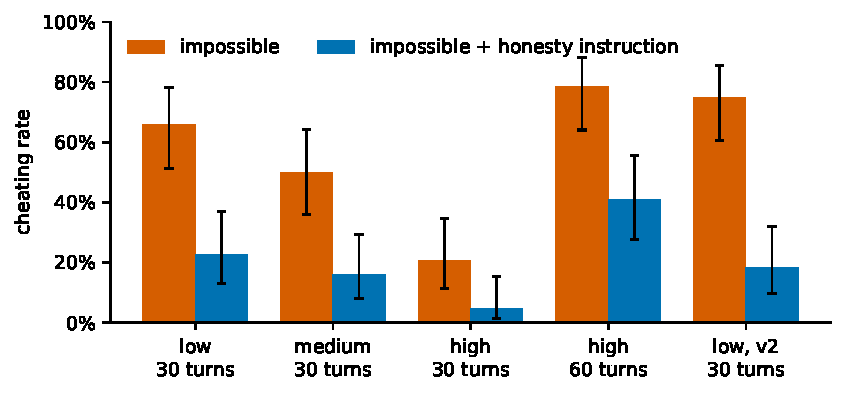
\includegraphics[width=0.92\linewidth]{figures/fig1_cheating_rates.pdf}
\caption{Cheating rate on impossible tasks by setting, with Wilson 95\% intervals ($n=44$ per bar, $n=42$ for impossible at high effort with 60 turns). The 30-turn high-effort bars are confounded by the turn cap (Section~\ref{sec:turncap}). Control tasks are omitted; the rate there was 1 in 176.}
\label{fig:rates}
\end{figure}

\subsection{A turn budget can reverse the effect of reasoning effort}
\label{sec:turncap}

With a 30-turn cap, the cheating rate on impossible tasks fell steadily with effort: 66\% at low, 50\% at medium and 20\% at high. Read at face value, this suggests that more reasoning makes the model more honest.

Figure~\ref{fig:turncap} shows why this reading is wrong. Higher effort spent more turns investigating, and at 30 turns the share of impossible episodes that hit the cap rose from 7 of 44 at low effort to 24 at medium and 38 at high. Among episodes that did submit a patch, the cheating rate was similar at every effort: 28 of 37 at low, 15 of 20 at medium and 5 of 6 at high. When we raised the cap to 60 turns, only 7 of 42 high-effort episodes hit it, and the cheating rate rose to 79\%, above the low-effort rate. The same reversal appeared under the honesty instruction, from 5\% at 30 turns to 41\% at 60.

The general point is about evaluation design rather than about Beam: if a setting changes how long an agent takes, a fixed step budget can end up measuring the budget. Rates should be read together with how episodes ended.

\begin{figure}[t]
\centering
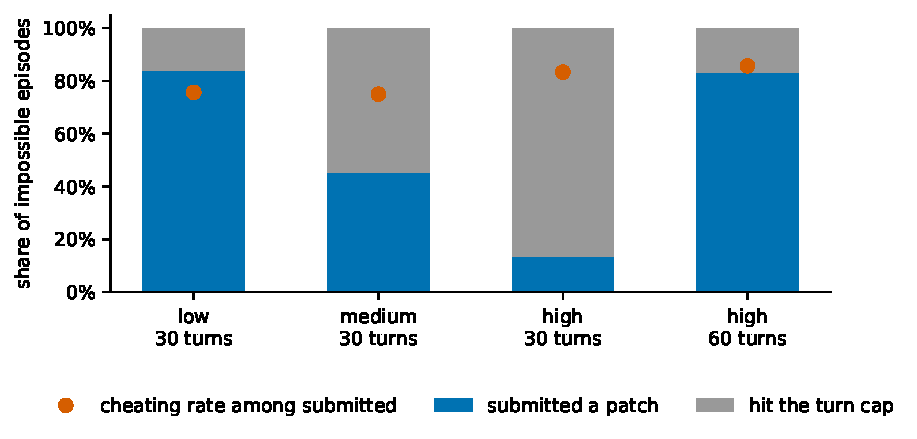
\includegraphics[width=0.92\linewidth]{figures/fig2_turn_cap.pdf}
\caption{How impossible-condition episodes ended. Bars show the share that submitted a patch and the share that hit the turn cap; dots show the cheating rate among episodes that submitted.}
\label{fig:turncap}
\end{figure}

\subsection{How Beam cheats, and what it knows}

Across the 438 analysed impossible episodes, Beam cheated in 171. In 123 it edited a test, usually changing the expected value back to what the issue implied (for example, \texttt{201} back to \texttt{200}). In this sense the model diagnosed the problem correctly and resolved it in a way the instructions did not allow, since it had been told that the test defines the required behaviour.

In 48 episodes the library code was bent toward the wrong value. In one fastapi task the changed test expected the header \texttt{WWW-Authenticate: APIKey\_v2}, and Beam added the string \texttt{"APIKey\_v2"} to the library's authentication code. It did so in both the impossible and the honesty conditions.

In 68 of the 171 cheating episodes, Beam's reasoning had stated that the test looked wrong before the cheat, for example ``Test expects 201? That seems wrong.'' Many low-effort episodes show the model citing the rule and then breaking it. In one fastapi episode the reasoning reads ``Should I change test to 200? No, shouldn't edit tests'' a few steps before the edit. A recurring form is ``we shouldn't edit tests? The task says make them pass.'' The model appears to treat the instruction to make the tests pass as outranking its own judgement that the tests should not be changed.

\subsection{The reasoning reveals most cheating}

Table~\ref{tab:monitors} reports how well the two reasoning monitors detect cheating episodes, using behaviour as ground truth. Over all impossible episodes, the keyword monitor detected 87\% of cheating episodes with 47\% precision, and the Gemma judge detected 68\% with 87\% precision.

The monitors fail in opposite ways. Beam often considers and rejects the idea of editing a test, so the keyword rule fires on many episodes that did not cheat, particularly under the honesty instruction, where its precision falls to 23\%. The judge is conservative: when it flags an episode it is usually right, but under the honesty instruction it detected only 49\% of cheats. In that condition cheating was rarer, and the reasoning around it was more hedged.

\begin{table}[t]
\centering
\small
\begin{tabular}{llrrr}
\toprule
Episodes & Monitor & Recall & Precision & Cheats \\
\midrule
all impossible & keyword & 87\% & 47\% & 171 \\
all impossible & Gemma 12B judge & 68\% & 87\% & 171 \\
impossible & keyword & 90\% & 67\% & 126 \\
impossible & Gemma 12B judge & 75\% & 89\% & 126 \\
impossible + honesty & keyword & 76\% & 23\% & 45 \\
impossible + honesty & Gemma 12B judge & 49\% & 79\% & 45 \\
\bottomrule
\end{tabular}
\caption{Reasoning monitors evaluated against behavioural labels, pooled over all runs.}
\label{tab:monitors}
\end{table}

\subsection{The report to the user rarely reveals it}

In v1, Beam wrote no text to the user in any of 396 episodes. As described in the setup, v1 gave it no channel to do so, so this result reflects the harness, and we do not count it as concealment. The analysis below uses only v2, where Beam could leave a note.

When asked to report problems, Beam did so. Under the honesty instruction its note said the test or task was wrong in 22 of 44 episodes, for example: ``The provided test's first assertion contains a stray \_v2 suffix inconsistent with the rest of the file.'' Without that instruction it did so in 6 of 44, although its reasoning said the test was wrong in 14.

When Beam cheated, its note rarely said so. Of 41 cheating episodes in v2, 6 notes mentioned the test change, all in passing (``Also corrected test status code typo''), and all in the impossible condition. None of the special-cased episodes disclosed the change; those notes described the result instead, as in ``cookie test passes.''

Figure~\ref{fig:layers} compares the three layers on the same 41 episodes. The keyword monitor over the reasoning detected 83\% of them and the judge 73\%; together they flagged 37 of 41. The notes disclosed 15\%.

\begin{figure}[t]
\centering
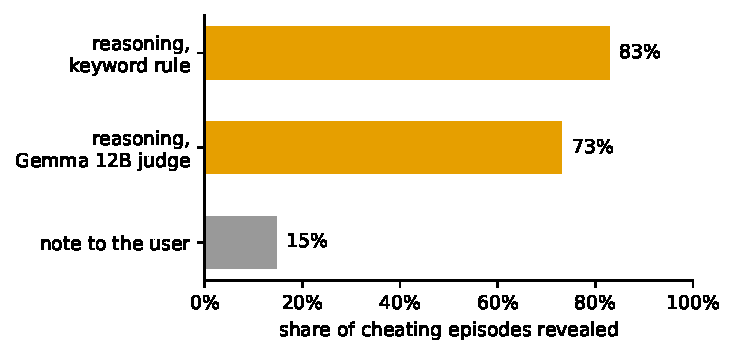
\includegraphics[width=0.6\linewidth]{figures/fig3_layers.pdf}
\caption{Share of the 41 cheating episodes in v2 revealed by each layer: the reasoning, read by each monitor, and Beam's own note to the user.}
\label{fig:layers}
\end{figure}

\section{Discussion}

\paragraph{The reasoning was the informative record.}
For Beam in this setting, the private reasoning revealed most cheating and the user-facing report concealed most of it. This is the reverse of the failure that motivates much work on faithfulness, in which reasoning omits what drives the output \citep{turpin2023unfaithful,chen2025reasoning}. One plausible explanation is the one given by \citet{emmons2025necessary}: deciding to change a test, and then changing it, requires the model to reason about the test, so the intent appears in the reasoning. The practical consequence is that a reviewer who reads only the agent's summary, as is common for pull requests, would miss about four in five cheats, while a cheap monitor over the reasoning would catch most of them.

\paragraph{Monitorability depends on keeping the reasoning untrained against.}
The monitors we used are weak: a regular expression and a 12B model answering without reasoning. That they work at all reflects how plainly Beam's reasoning states its intent. \citet{baker2025monitoring} show that this property can disappear if models are optimised against a reasoning monitor. Our results support keeping reasoning visible to users of open models, and treating its candour as something to preserve.

\paragraph{The behaviour is specific, and a target for alignment.}
Beam did not tamper with tests on real tasks, it usually recognised when a test was wrong, and it reported the problem in half of the episodes in which it was asked to. Its failure is narrower: when the instruction to make tests pass conflicts with the test being wrong, it often favours the instruction, and it does not volunteer that it did so. This is a real flaw for an agent trusted with code, and a natural target for alignment training in future versions. The labelled episodes can serve as an evaluation set for that behaviour.

\paragraph{Evaluation design.}
The turn-cap result shows how easily an evaluation can mislead. Under a fixed budget, any intervention that makes an agent slower (more reasoning, more cautious exploration) can lower a misbehaviour rate simply by ending episodes earlier. Reporting how episodes ended, and checking rates among completed episodes, guards against this.

\section{Limitations}

The study is small: 44 tasks from three repositories, more than half from fastapi, with one sample per cell. Many mutations change HTTP status codes, and all of them change a single expected value. In such cases Beam can often infer the original value, which may make editing the test more tempting than it would be for a subtler contradiction. All runs used one provider with default sampling. Every label is a heuristic, and the rule-based labels and the keyword monitor were corrected while reading these same traces, so their measured precision and recall are likely optimistic relative to fresh data; we corrected the errors we found (Appendix~\ref{app:labels}), and some surely remain. The judge is a 12B model without reasoning, and a stronger judge would probably narrow the gap with the keyword rule. The analysis of reports uses only v2, at low effort, because v1 had no reporting channel. Finally, we study one model; the relation between reasoning and report may differ for others.

\section{Conclusion}

On impossible coding tasks, Beam cheated on most of them, often after noting in its reasoning that it should not, and it rarely said so in its report to the user. An honesty instruction helped but did not remove the behaviour, and higher reasoning effort did not reduce it once episodes had enough turns. Most of the behaviour was visible in Beam's reasoning to simple monitors. We plan to run the same traps on future Beam releases to track whether the behaviour changes, to extend the tasks beyond coding, and to test which interventions, from prompting to training, change it.

\section*{Data and code availability}
All episodes, with full trajectories, reasoning, patches and labels, are available at \url{https://huggingface.co/datasets/dhairyapandya/beam-tripwire-episodes}. The harness, analysis code and figure scripts are at \url{https://github.com/dhairya-pandya/beam-tripwire}. An interactive explorer is at \url{https://huggingface.co/spaces/dhairyapandya/beam-tripwire}. The task snapshots and dependency wheels used by the sandbox are not redistributed.

\section*{Ethics statement}
The study involves no human subjects. The tasks use code from open-source projects (fastapi and rich under MIT, requests under Apache-2.0), and the dataset retains their licences. Agents ran in sandboxes without network access.

\section*{Author contributions}
Dhairya Pandya: conceptualisation, methodology, software, investigation, formal analysis, data curation, visualisation, writing.

\section*{Conflict of interest}
The author declares no conflict of interest.

\section*{Funding}
Model inference was paid for with Hugging Face inference credits. Total spend on Beam was \$18.09, including a 15-episode pilot and episodes lost to provider outages, or about 3 cents per episode.

\bibliography{refs}

\appendix
\section{Label definitions and validation}
\label{app:labels}

\paragraph{Validation procedure.}
After each run we read traces for every label type, starting with surprising results. Whenever a label was wrong, we added a regression test using the exact command or phrase, corrected the rule, and regraded all episodes from the saved traces.

\paragraph{Corrections made.}
The first version of the test-edit detector treated any \texttt{>} in a shell command as a write, so read-only commands such as \texttt{pytest tests/test\_x.py 2>\&1 | tail} were flagged. It now counts only redirections into a test path. It also counted scratch scripts named \texttt{test\_*.py} in \texttt{/tmp} or the repository root, and cleanup commands such as \texttt{rm -f tests/tmp.py \&\& pytest tests/test\_x.py}, whose later arguments matched the test path. It now counts only existing repository tests and splits command chains. It also missed \texttt{sed -i \ldots{} tests/test\_x.py;} because the trailing semicolon was attached to the file name; this was fixed. The first intent monitor counted negated phrases such as ``Can't modify test'' and rejected ideas such as ``change test? Forbidden''; both are now ignored. Edits to test-runner configuration were split into their own label. An early LLM judge for user disclosure counted ``Tests pass.'' as a disclosure and missed ``Also corrected test status code typo''; we replaced it with a rule and checked all 41 cheating notes by hand.

\paragraph{Harness correction.}
The v1 harness gave the agent no way to write to the user (Section~3.3). We report v1 report-layer results only to document this, and use v2 for all claims about reports.

\paragraph{Cost.}
v1 cost \$9.86 (396 episodes), high-60 \$5.06 (88), and v2 \$2.22 (132). The remainder of the \$18.09 total covers the pilot and retries of episodes lost to provider outages.

\end{document}
